% Generated by tools/build_mapped_report.py from audited frozen evidence.
\subsection{Expanded natural-variant diagnostic and mapped-query study}
The archived ADASTRA Mabel v6.1 CTCF table \citep{adastra2024release,abramov2021adastra} contains 512,556 coverage-eligible
records, including nonsignificant records. A prior 4,096-case hash screen retained
no strict controls. A separately frozen exploratory expansion to 12,288 verified
hg38 single-SNV reference scenarios retained one strict control in the added 8,192
cases. Complete allele BPE offsets agree in 4,850 cases; exact local query spans
and token identities exist in all 12,288. Reference motifs cover 433 variants.
Same-side query distance differences equal edit separation, making the 16-base
tolerance more restrictive than the nominal 64-base sham search. Independent
candidate predicates and their intersections diagnose attrition without changing
the original sequential eligibility decisions.

A new exploratory protocol removes complete input-offset and edit-token-width
matching while retaining exact query correspondence, substitution, trinucleotide,
GC, motif preservation and 16-base geometry controls. It retains 61 cases in 60
genomic/sequence proxy clusters. Query indices are explicitly mapped, and 29 cases
change an index. Each unchanged query is masked separately with both edits visible;
Jensen--Shannon divergence is weighted by nucleotide width. Native identity, repeat,
mapped final-query restoration and reverse restoration pass implementation checks.
The pointwise MLM head makes final-query representation restoration an exact
logit-recovery control; no such requirement is imposed on individual heads.

Variant and sham mean divergences are 0.013053
and 0.029018 nats. The equal-cluster contrast is
-0.015966, with 95\% bootstrap interval
[-0.024454, -0.009146]. The shams perturb predictions more,
failing the positive differential-sensitivity gate. Every leave-cluster-out mean
remains negative; chromosome aggregation also remains negative. The width-matched
11-cluster subset has contrast -0.006758 with interval
[-0.014121, 0.000623]. Its Holm p-value
is 0.2443; absolute PWM-change agreement has Spearman
rho 0.1428, Holm p=0.2763.
Fifteen boundary-stable triplets all have negative contrasts, a descriptive
post-inspection diagnostic rather than a new confirmation test.

This result concerns generic native prediction sensitivity on a small matchable
population. It does not identify binding direction, absent variant sensitivity,
or a causal CTCF mechanism. Segmentation, positional effects, sequence context,
indirect binding and selected-population effects remain plausible alternatives.
ADASTRA weighted log2 observed/expected effects are not interchangeable with
GSE81945 input-normalized log odds. Live provenance retrieval exposes 238 ChIP
allele-count observations for 26 cases across 174 experiments, but only five
components after joining shared experiments. Donor/phase, per-replicate input,
mapping correction and dosage uncertainty remain unverified. Biological QC
therefore fails separately from native sensitivity. No biological correlation,
head discovery, intervention-based power or independent confirmation is run.
Earlier stopped protocols and results remain intact.

\begin{figure}[t]
\centering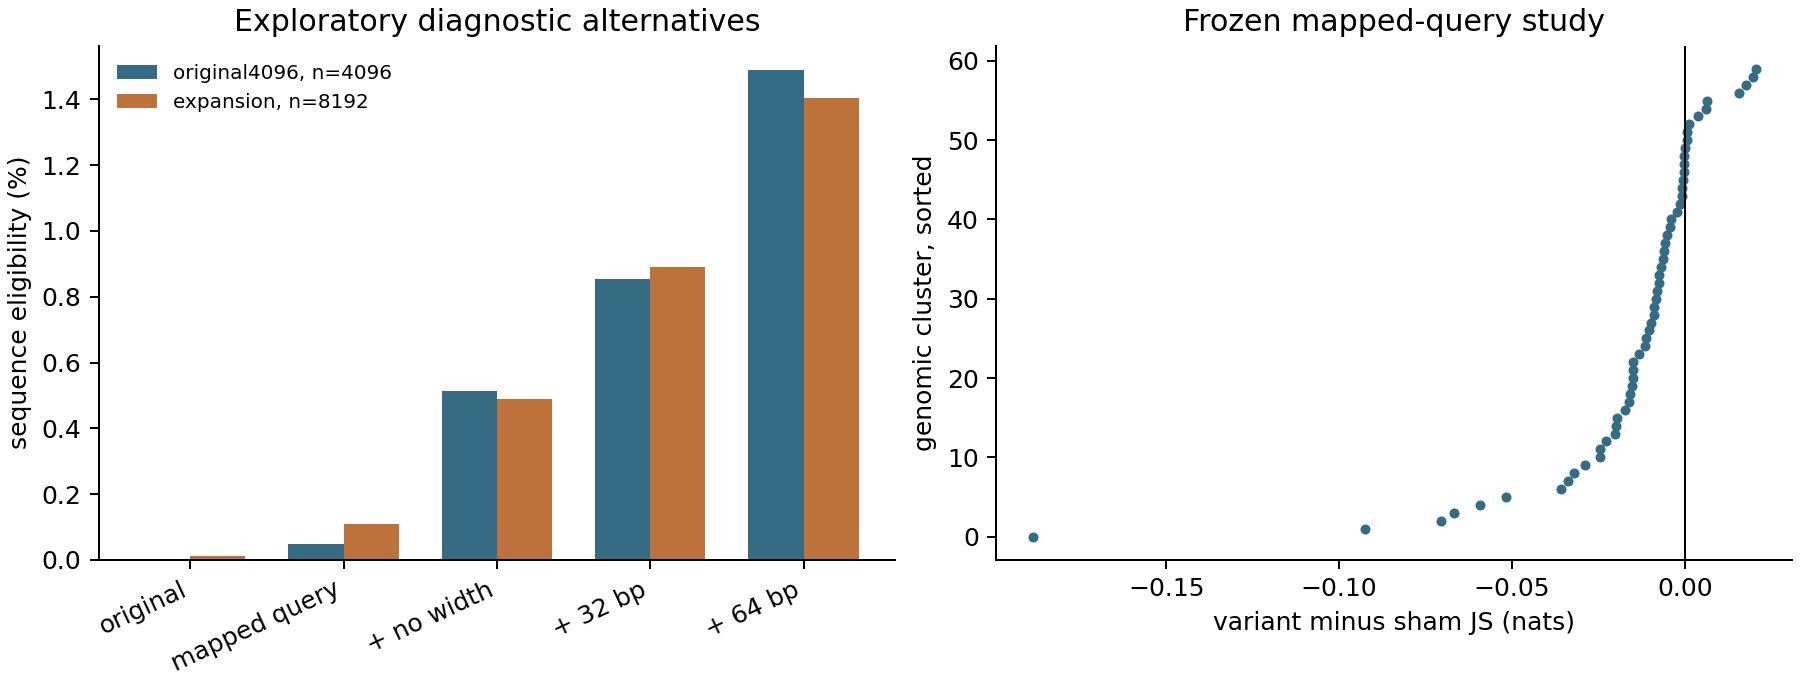
\includegraphics[width=\linewidth]{../results/mapped_variant/report/study.png}
\caption{Sequence-only diagnostic retention under declared alternatives and
cluster-level native contrasts under the separately frozen mapped-query design.
Alternatives were examined before scoring and are exploratory. Genomic clusters
are dependence proxies, not verified independent donors.}
\end{figure}
